% !TeX spellcheck = fr_FR
\begin{resume}
La gestion de l'hétérogénéité des ressources peut être considérée sous plusieurs aspects. Les chapitres précédents ont donné des exemples de travaux dans lesquels l'hétérogénéité s'était concentrée sur les communications (Chapitre \ref{Chap:MPI}) ou sur le couple données-communication (Chapitre \ref{SEC:GRAPPES}). Dans ce chapitre nous nous concentrons sur un troisième socle, celui de l'hétérogénéité du calcul. Plus exactement, ce chapitre présente des travaux dont les contributions ont visé la prise en charge de l'hétérogénéité des ressources de calcul ou l'hétérogénéité des tâches de calcul, tous les deux résultant en une variabilité des temps d'exécution de tâches qui a dû être traitée et optimisée. Il est aussi important de remarquer que la communication et le stockage peuvent varier mais, dans ces cas, ils sont traités par des outils et mécanismes subjacents qui n'ont pas été la cible de nos travaux.

Ainsi, ce chapitre démarre avec la description d'une plate-forme de calcul destinée à l'exécution de problèmes d'amarrage moléculaire. Ce travail, développé dans le cadre de la codirection de thèse de Romain Vasseur, est un exemple d'application métier où l'environnement développée sert à déployer de manière distribuée une application déjà existante et dont le code source ne pourrait pas être facilement parallélisée. L'approche retenue a été composée d'une gestion distribuée d'instances de calcul sur un cluster, associée à un découpage plus fin du problème afin de multiplier les tâches de calcul et ainsi mieux utiliser les ressources disponibles.

La deuxième partie de ce chapitre décrit les efforts effectués dans le cadre du projet de collaboration international STIC-AmSud PER-MARE, dont l'un des objectifs a été de rendre la plateforme de calcul \textit{big data} Hadoop sensible au contexte et donc capable d'adapter la distribution des tâches de calcul en fonction des variations des ressources.

\end{resume}

\section{Hétérogénéité des Tâches  - application à la recherche en amarrage moléculaire} \label{sec:Vasseur}

L'utilisation d'approches informatiques pour identifier les interactions biomoléculaires est devenu l'un des principaux piliers de la recherche de nouvelles drogues et principes actifs. En effet, la simulation \emph{in silico} permet de faire une première prospection sur un grand nombre de candidats potentiels, tout avec un gain de temps important et un coût nettement moins onéreux que l'expérimentation \emph{in vitro}. 

L'amarrage moléculaire (aussi appelé \emph{docking moléculaire}) est donc une technique qui vise à étudier les interactions au niveau moléculaire entre certaines structures du vivant, comme par exemple les interactions protéine-ADN/ARN, protéine-protéine, peptides-protéine, protéine-ligand ou glucide-protéine. L'industrie pharmaceutique s'intéresse particulièrement à l'étude des interactions protéine-ligand, notamment la recherche de principes actifs de médicaments (ligands) qui puissent se connecter à certaines protéines cible. La prédiction des modes d'amarrage d'un ligand à une protéine, la structure du complexe résultant et l'estimation de l'affinité de cet amarrage sont essentiels pour le développement de nouveaux composés thérapeutiques, et les méthodes numériques ont été le choix principal de plusieurs travaux dans la littérature \cite{Abagyan2001,Giganti2010, Klebe2006}.

 Souvent cette étude se fait à travers un "criblage virtuel" (\emph{virtual screening}), qui consiste en un déploiement à grande échelle permettant de tester un grand nombre de ligands (de centaines à plusieurs millions selon l'ampleur de la campagne) sur un nombre très restreint de cibles. En effet, nous trouvons des millions de composants catalogués dans des bases de données telles que la Cambridge Structural Database \cite{Allen2002}, PDBbind  \cite{Wang2004, Wang2005}, ZINC \cite{Irwin2005} et tant d'autres collections privées des groupes pharmaceutiques. De même, un riche catalogue de protéines peut être obtenu à partir du Research Collaboratory for Structural Biology (RCSB) Protein Data Bank (PDB) \cite{PDB}, une base de données ouverte qui contient plus de 120 000 protéines cataloguées et qui est enrichie de plus de 7000 nouvelles protéines par an. Ainsi, un chercheur ou un industriel qui souhaite activer ou désactiver une protéine afin de combattre une maladie peut donc effectuer ce criblage virtuel entre la protéine cible et les milliers de ligands catalogués (enzymes, peptides, etc.).  

Dans le cadre des travaux de thèse de Romain Vasseur (thèse en bio-informatique, dirigée par le prof. Manuel Dauchez et co-encadré par Stéphanie Baud et moi-même) nous nous sommes penchés sur le développement et l'exécution parallèle d'une application pour le criblage moléculaire inversé. Plus exactement, un criblage inversé a pour objectif de discriminer les cibles protéiques les plus favorables à une interaction avec le ligand, parmi un échantillon de structures de protéines plus ou moins important. De cette manière, il est possible d'identifier des cibles secondaires pour un ligand développé, ou bien faire une étude préalable des risques d'interactions indésirables. 

\subsection{Travaux Proches et Méthodologie de Parallélisation}

Le terme \textit{inverse docking} a fait son apparition dans la littérature en 2001 avec les deux articles de Chen \textit{et al}. \cite{Chen2001,Chen2001b}. Une quinzaine d'articles ont été recensés depuis cette date, avec des méthodes de traitement à plus ou moins grande échelle. La plupart de ces travaux font l'usage d'applications pour le docking traditionnel telles que AutoDock \cite{Steffen07} ou AutoDock Vina \cite{Lauro2011,Lauro2012}, avec très peu d'outils dédiés exclusivement au docking inversé (INVDOCK \cite{Chen2001,Chen2001b} ou TarFisDock \cite{Li2006}). Toutefois, aucun de ces articles ne décrit ni ne mentionne le développement d'une méthode de déploiement sur des architectures de type HPC.

Ainsi, nous avons développé nos propres stratégies dans le but de pouvoir traiter des centaines en parallèle de protéines grâce aux architectures HPC.
Ces stratégies concernent la parallélisation du calcul d'un couple ligand-protéine mais aussi le déploiement large échelle de ces calculs. 

Dans ce travail nous sommes parti de la méthode appelée \textit{blind docking} qui consiste à détecter des points d'amarrage possibles en faisant un balayage sur l'ensemble de la surface de la protéine. Pour cela, des applications telles que Autodock doivent générer une grille d'affinités basée sur les énergies de liaison de chaque atome qui compose la protéine. Cette grille d'affinité se présente comme une boîte 3D qui contient toute la surface de la protéine, plus une marge afin de permettre le placement d'un ligand à l'intérieur de la boîte. Par la suite, un algorithme génétique ira explorer le volume autour de la protéine afin d'évaluer l'énergie de liaison à différents endroits. 

L'approche \textit{blind docking} est naïve et difficilement parallélisable car chaque pair protéine-ligand représente une boîte et donc une tâche de calcul Autodock. De plus, selon les caractéristiques de la protéine, un nombre important d'itérations (générations dans l'algorithme génétique) sont nécessaires pour couvrir systématiquement la surface de la protéine et permettre l'obtention de résultats satisfaisants. Comme résultat, l'exécution d'une seule instance du \textit{blind docking} avec l'application AutoDock peut prendre plusieurs heures. Malgré ces contraintes, cette approche est assez répandue et a donc été utilisée comme référence de comparaison pour les approches parallèles que nous avons développées.

\subsection{Parallélisme Intérieur : décomposition des tâches}
Afin d'optimiser l'utilisation des ressources de calcul lors d'une campagne de docking inversé, il est impératif d'intégrer le parallélisme au c{\oe}ur du traitement des tâches de calcul, comme illustré en figure \ref{fig:romain-fig1}. La décomposition d'une instance de docking permet une meilleure utilisation des ressources de calcul en distribuant les tâches sur plusieurs machines, mais aussi grâce à un traitement en pipeline qui permet l'enchaînement des opérations lorsque certaines tâches finissent plus tôt. De plus, cela rend l'exécution plus tolérante aux fautes, une tâche qui a été interrompue peut être redéployée sur une autre machine sans obliger le redémarrage de toute l'exécution. Dans le cadre de ce travail, nous avons étudié les techniques de décomposition présentées dans les sections suivantes. 

\begin{figure}
	\centering
		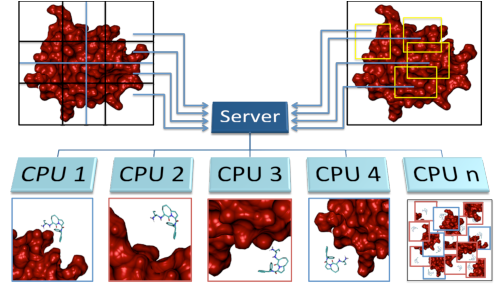
\includegraphics[width=0.5\linewidth]{images/Romain/fig1-color}
	\caption{Exemple d'un schéma de décomposition parallèle}\label{fig:romain-fig1}
\end{figure}

\subsubsection{Décomposition géométrique arbitraire}
Vu la nature des données utilisées en entrée pour le docking, nous avons initialement étudié une stratégie de décomposition géométrique qui consiste à découper la grille d'affinité 3D en plusieurs boîtes plus petites, chacune couvrant un secteur de la protéine. Cette stratégie considère une décomposition géographique régulière de telle manière que le nombre de tâches (boîtes) ont une taille similaire, permettant ainsi la génération de $n^3$ sous-grilles : 8 (2x2x2), 27 (3x3x3), 64 (4x4x4), etc. Le choix du bon nombre de découpages dépend à la fois du gain  en parallélisme mais aussi de la liberté de mouvement du ligand à l'intérieur d'une grille. 
En effet, on peut espérer un gain de performance du fait de pouvoir déployer en parallèle les différentes sous-grilles comme des tâches de calcul indépendantes. Toutefois, un nombre trop important de découpages aura pour effet la génération de sous-grilles "inutiles" car elles couvrent que des zones inaptes à la recherche de points d'amarrage (espace non connecté à la surface de la protéine, "intérieur" de la protéine, etc.). De plus, une boîte 3D trop petite peut empêcher le positionnement du ligand et donc rendre l'évaluation de l'amarrage impossible.

Un autre inconvénient de cette technique est que le découpage se fait de manière arbitraire, sans prendre en compte les spécificités de la surface de la protéine. Par exemple, les "cavités" présentes dans la surface de la protéine sont souvent des bons sites pour l'amarrage, mais un découpage arbitraire qui l'ignore peut simplement scinder cette cavité en deux et la rendre bien moins intéressante vis-à-vis de l'algorithme de docking. De même, l'évaluation de docking se fait en considérant que le ligand se trouve totalement à l'intérieur de la sous-grille : n'importe quelle conformation où des atomes ligand dépassent la grille serait invalide et donc ignorée. 

\subsubsection{Décomposition géométrique avec superposition}
Les inconvénients de la décomposition géométrique arbitraire cités dans la section précédente nous ont conduit à développer une technique alternative de découpage qui préserve la liberté de placement des ligands et permet une couverture intégrale de la surface de la protéine. Cette technique consiste à effectuer un découpage avec superposition entre les sous-grilles voisines, de manière à pouvoir évaluer le placement du ligand même sur les zones proches des bords des sous-grilles. Bien sûr, cette superposition est dépendante de la taille des ligands, permettant ainsi une configuration qui optimise l'utilisation des ressources pour chaque pair protéine-ligand. 

Ainsi, dans le cadre du travail effectué, nous avons considéré deux valeurs de référence pour la superposition. La superposition entre deux boîtes serait d'un tiers de la longueur de la boîte si la longueur du ligand est inférieure à cela. Dans le cas contraire, la superposition correspond à la longueur du ligand. Grâce à cette configuration, le ligand a une liberté complète de placement (rotation, translation, etc.) et on peut effectuer une recherche exhaustive sur l'espace d'amarrage. Dans l'exemple illustré dans les prochaines sections nous utilisons aussi un schéma de décomposition en douze parties, 3x2x2 (où 3 correspond à l'axe principal de la protéine) et avec une superposition d'1/3 sur chaque sous-grille. 

\subsubsection{Recherche de cavités}
Comme indiqué précédemment, l'amarrage des ligands est favorisé par la présence de cavités dans la surface de la protéine \cite{Ghersi2009,Hetenyi2011}, or les méthodes de découpage par décomposition ne prennent pas ces facteurs en compte. En effet, même avec la décomposition avec superposition, l'algorithme génétique utilisé pour la recherche de points d'amarrage ne fait que parcourir la surface sans un objectif précis. 

Nous pouvons améliorer la précision de notre docking inversé en effectuant la détection des zones avec cavités, par exemple à l'aide d'un programme dédié à ce fin, l'application Fpocket \cite{Guilloux09a}. La prise en compte des zones avec un plus grand potentiel peut augmenter la performance du docking inversé car cela nous permet de concentrer la recherche sur une zone plus spécifique. L'inconvénient est que son application nécessite un réglage fin des paramètres afin d'inclure les spécificités des protéines et de ne pas exclure des zones avec un potentiel moindre mais réel. 

Ainsi, au lieu de se reposer uniquement sur la recherche de cavités, notre travail a misé sur la complémentarité entre celle-ci et la décomposition géométrique avec superposition. En plus de générer des tâches de calcul pour les différentes sous-grilles issues de la décomposition géométrique, nous générons aussi des recherches ciblées sur les cavités identifiées par FPocket. Ces paramètres permettent une meilleure couverture des zones avec un plus grand potentiel (car couvertes par les deux techniques), tout en limitant le nombre de tâches de calcul supplémentaires.


\subsection{Gestion et Déploiement des Tâches de Calcul}

Les techniques de découpage présentées dans la section précédente permettent la parallélisation du traitement d'un couple protéine-ligand. Dans le cas du docking inversé, ce parallélisme dit "interne" doit être associé à la génération et au traitement des multiples tâches de calcul issues de chaque combinaison entre un ligand cible et la base de données de protéines recherchée. Enfin, les tâches de préparation des données (génération des sous-grilles, définition des paramètres, regroupement des résultats, etc.) doivent aussi être prises en compte. 

Pour toutes ces raisons, nous avons créé deux implémentations visant la gestion et le déploiement des tâches, toutes les deux intégrées à l'outil AMIDE \cite{Vasseur2015}. Dans le premier cas, une plate-forme générique qui gère tout seule l'ensemble des tâches a été conçue. Dans le deuxième cas, une partie des responsabilités est déléguée aux gestionnaires de tâches des clusters, simplifiant ainsi son exécution dans les environnements déjà pourvus de tels outils.

\subsubsection{Plate-forme générique}

Vu les besoins de parallélisme interne et externe, nous avons dans un premier moment spécifié et développé une plate-forme générique basée sur le langage Python et capable d'exploiter le parallélisme multi-c{\oe}ur et multi-machine pour le docking inversé. 

Ainsi, un ensemble de scripts Python a été créé afin d'automatiser toutes les étapes liées à la préparation et à l'exécution du docking inversé. Parmi ces étapes nous pouvons citer :
\begin{itemize}
	\item[\textbf{(i)}] l'acquisition des fichiers PDB qui décrivent les protéines et ligands, 
	\item[\textbf{(ii)}] la préparation des fichiers PDB afin de sélectionner les structures cible, 
	\item[\textbf{(iii)}] l'extraction des coordonnées pour la création des grilles d'affinité, 
	\item[\textbf{(iv)}] la décomposition des grilles et 
	\item[\textbf{(v)}] le déploiement des tâches de calcul. 
\end{itemize}

Les étapes (i) et (ii) concernent majoritairement la manipulation de fichiers et le parsing des informations, alors que les étapes  (iii) et (iv) sont liées à l'exécution de Autogrid, un outil qui fait partie de la suite Autodock et qui permet la création des grilles pour le docking. Selon la stratégie de décomposition retenue, l'étape (iv) peut créer une ou plusieurs grilles correspondant au découpage 3D. Dans le cas de l'approche par recherche de cavités, des grilles 3D sont généré uniquement autour des zones identifiées par le logiciel Fpocket. 


\begin{figure}
	\centering
		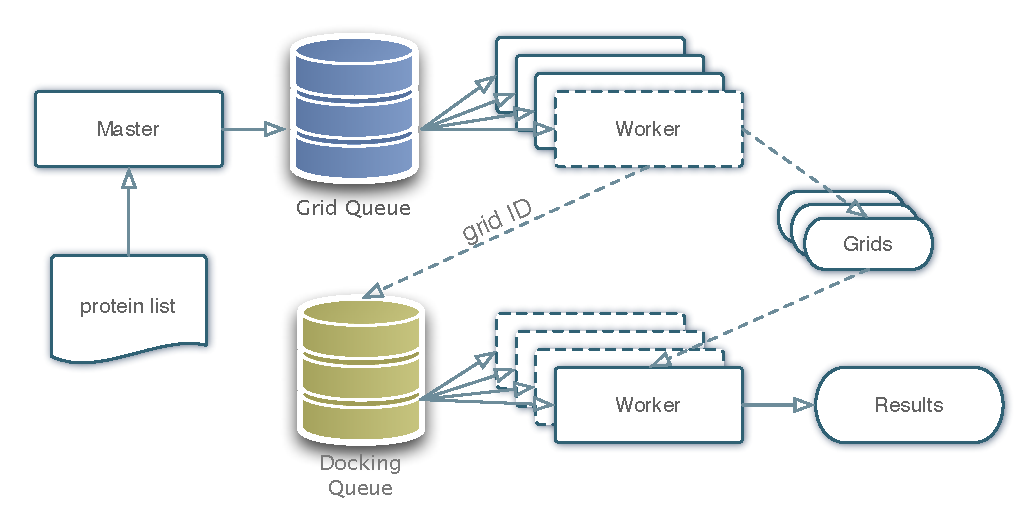
\includegraphics[width=0.5\linewidth]{images/Romain/fig3-color}
	\caption{Représentation du flot d'exécution dans l'architecture distribuée}\label{fig:romain-fig3}
\end{figure}


Pour cela, la plate-forme utilise une architecture distribuée maître-esclave avec gestion d'une file d'exécution contenant les identifiants des tâches (task ID) et accessible en mode "sac de tâches" (\textit{bag of tasks} en anglais). Grâce à cette stratégie, les différents esclaves obtiennent une ou plusieurs tâches à exécuter, selon le nombre de c{\oe}urs de calcul disponibles. Pour être plus exacte, dans cette architecture nous trouvons deux files d'exécution, l'une dédiée à la préparation des sous-grilles et l'autre dédiée à l'exécution des tâches de docking. La première file est alimentée par le maître qui, à partir des paramètres d'entrée, indique aux esclaves les différentes protéines à analyser et aussi les stratégies de découpage à mettre en place, ainsi que la génération des sous-grilles avec l'outil Autogrill de la suite Autodock. Les esclaves doivent d'abord finir toutes les tâches dans cette file avant de passer à la file suivante.

Pour plus d'efficacité, la deuxième file d'exécution n'est plus alimentée par le maître mais directement par les esclaves. Lorsque ceux-ci finissent la préparation d'une tâche de la première file, il suffit de déposer le TaskID correspondant dans la deuxième file d'exécution. La Figure \ref{fig:romain-fig3} illustre le flot d'exécution de ces deux étapes.  


\subsubsection{Optimisation aux clusters HPC}

 L'architecture distribuée présentée ci-dessous est adaptée à une exécution sur tout type de réseau d'ordinateurs (cluster, cloud, grid pervasif, etc.). Toutefois, il est possible d'optimiser son fonctionnement sur les clusters HPC si on prend en compte l'existence d'un gestionnaire de tâches propre à ces systèmes. En effet, la plupart des clusters HPC fait l'usage d'un gestionnaire de tâches afin de garantir la réservation et l'équité d'usage des ressources. Des systèmes tels que PBS \cite{Henderson95}, OAR \cite{Capit2005} ou Slurm \cite{Yoo2003} sont capables de gérer plusieurs files d'exécution ainsi que de déployer des tâches en mode \textit{best effort} de manière à occuper les ressources de calcul lorsque les réservations ne suffisent pas. 
 
 Dans le cas de l'optimisation pour les clusters HPC notre stratégie a été d'éliminer la dépendance vis-à-vis d'un n{\oe}ud maître et permettre ainsi l'exécution des tâches indépendantes selon les disponibilités du gestionnaire de tâches. En effet, la présence d'un n{\oe}ud maître était nécessaire afin de gérer les files d'exécution mais aussi de vérifier la terminaison des tâches (garantissant la tolérance aux fautes). Cela oblige donc que le processus maître reste actif pendant toute l'exécution, ce qui impose des problèmes lors de la réservation des ressources destinées au maître (combien de temps faut-il le garder actif ?). Cette limitation est encore plus importante dans le cas d'un déploiement \textit{best-effort}, où la terminaison des tâches risque d'être fortement étalée au gré de l'occupation des ressources. Comme les gestionnaires de tâches des clusters HPC sont capables de détecter une tâche interrompue et la relancer, il suffit de soumettre dans une même tâche les paramètres nécessaires à la génération des sous-grilles et à leur docking. 
 
 Grâce à cette optimisation, l'outil AMIDE issu de ces travaux est capable d'effectuer le docking inversé autant dans un cluster que dans un agglomérat de machines indépendantes.
 
 \subsection{Évaluation Pratique}
 
 Lors de la mise en place de l'outil AMIDE nous avons exécuté plusieurs expériences dans le but de valider notre approche de travail. L'un de ces tests consistait à évaluer la précision des stratégies de décomposition en étudiant un complexe ligand(X23)-protéine(3CM2) bien connu dans la littérature. La comparaison s'est fait par rapport à la technique classique du \textit{blind docking} mais aussi par rapport à des données expérimentales obtenues par cristallographie. Dans un deuxième moment, nous avons conduit des tests de performance dans lesquels le docking inverse était déployé sur un large ensemble de protéines issues de la bibliothèque PDB.
 
Toutes les expériences ont été conduites sur le cluster Clovis du centre de calcul ROMEO à Reims. Clovis était un cluster hybride avec 36 n{\oe}uds Westmere-EP (12 c{\oe}urs), 2 n{\oe}uds Nehalem-EX (32 c{\oe}urs), un n{\oe}ud Westmere-EP (12 c{\oe}urs + 2 Fermi C2050 GPUs) et un n{\oe}ud Nehalem-EP (8 c{\oe}urs + GPU Fermi M2090), et au moins 2GB de mémoire par c{\oe}ur. Pour une question de régularité, les expériences ici présentées ont été lancées exclusivement sur les n{\oe}uds Westmere-EP. De plus, afin de mieux évaluer la communication intra-cluster, seulement 4 c{\oe}urs de calcul ont été utilisés par n{\oe}ud.
 
 Ainsi, pour la première expérience, nous avons initialement exécuté un blind docking de la protéine 3CM2 et du ligand X23. Comme illustré en  Figure \ref{fig:blind}, le blind docking a permis la détection de la cavité et d'une conformation presque identique à celle obtenue par cristallographie (différence RMSD de 1.60 Angstroms seulement).
 
 \begin{figure}[h]
 	\centering
 		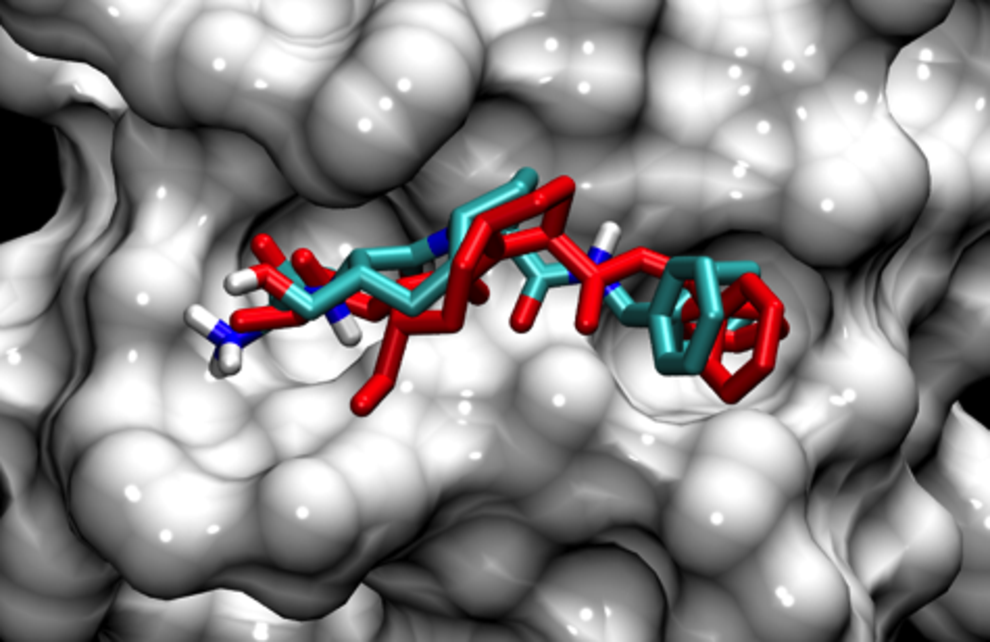
\includegraphics[width=0.85\linewidth]{images/Romain/fig4-color} 
 		\caption{Placement du ligand selon la méthode cristallographique (rouge) et par blind docking (vert)}\label{fig:blind} %\vspace{-0.3cm}
 \end{figure}
 
 \begin{table}
 	\begin{center}
 		\caption{Tableau comparatif des précisions du docking de 3CM2 selon les stratégies de décomposition et le nombre d'itérations. La distance RMSD est comparée à la pose cristallographique et les énergies de liaison à celles obtenues par la méthode blind docking.}\label{tab:rmsd}
 		\begin{tabular}{|c|c|c|c|}
 			\hline 
 			$\Delta G$ blind docking & Nombre d'itérations & énergie de liaison $\Delta G$ & RMSD  \\ 
 			($kcal.mol^{-1}$)  &  & ($kcal.mol^{-1}$) &  (\AA{}) \\
 			\hline 
 			\multirow{3}{*}{$\Delta G = -10.27$}  & 20 & $\Delta G_{12} = -10.09$ & 1.79 \\ \cline{2-4}
 			& 50 & $\Delta G_{pocket} = -10.11$ & 1.86 \\ \cline{2-4}
 			& 70 & $\Delta G_{pocket} = -10.39$ & 1.62 \\ \cline{2-4}
 			\hline 
 		\end{tabular} 
 	\end{center}
 	%\vspace{-0.3cm}
 \end{table}
 
Le découpage avec le meilleur score d'énergie de liaison est celui en $n = 12$, comme illustré en Figure \ref{fig:cuts}. Avec seulement 20 itérations, ce type de décomposition a permis l'obtention d'un placement similaire à celui de la méthode blind docking (voir Table \ref{tab:rmsd}). Les autres formats de découpage ont réussi à placer le ligand dans la cavité cible, mais leurs résultats en termes d'énergie de liaison et de distance RMSD ne sont pas suffisants. La méthode de recherche de cavités a aussi permis le placement du ligand avec une bonne précision, au bout de 50 itérations. 


 
 \begin{figure}[h]
 	\centering
 		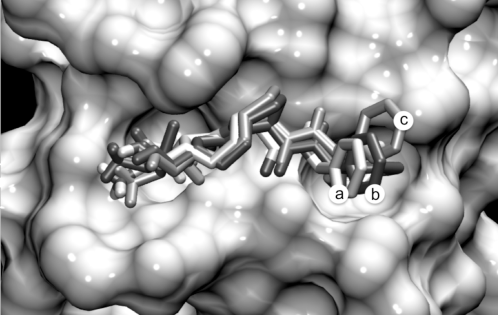
\includegraphics[width=0.85\linewidth]{images/Romain/fig5-bw} 
 		\caption{Comparaison entre la pose blind docking (a) et celle d'un découpage à $n=12$ (b) et par recherche de cavités (c). }\label{fig:cuts} %\vspace{-0.3cm}
 \end{figure}

\begin{figure}
	\centering
		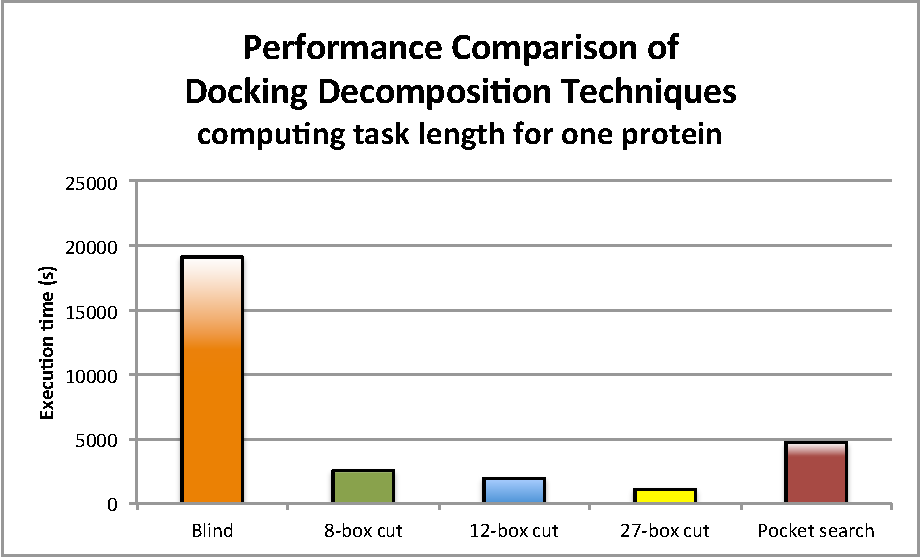
\includegraphics[width=0.5\linewidth]{images/Romain/fig7-color}
		\caption{Comparaison des temps d'exécution pour les tâches issues des différentes méthodes de découpage}\label{fig:performance} %\vspace{-0.3cm}

\end{figure}

%\begin{figure}[h]
%	\begin{center}
%		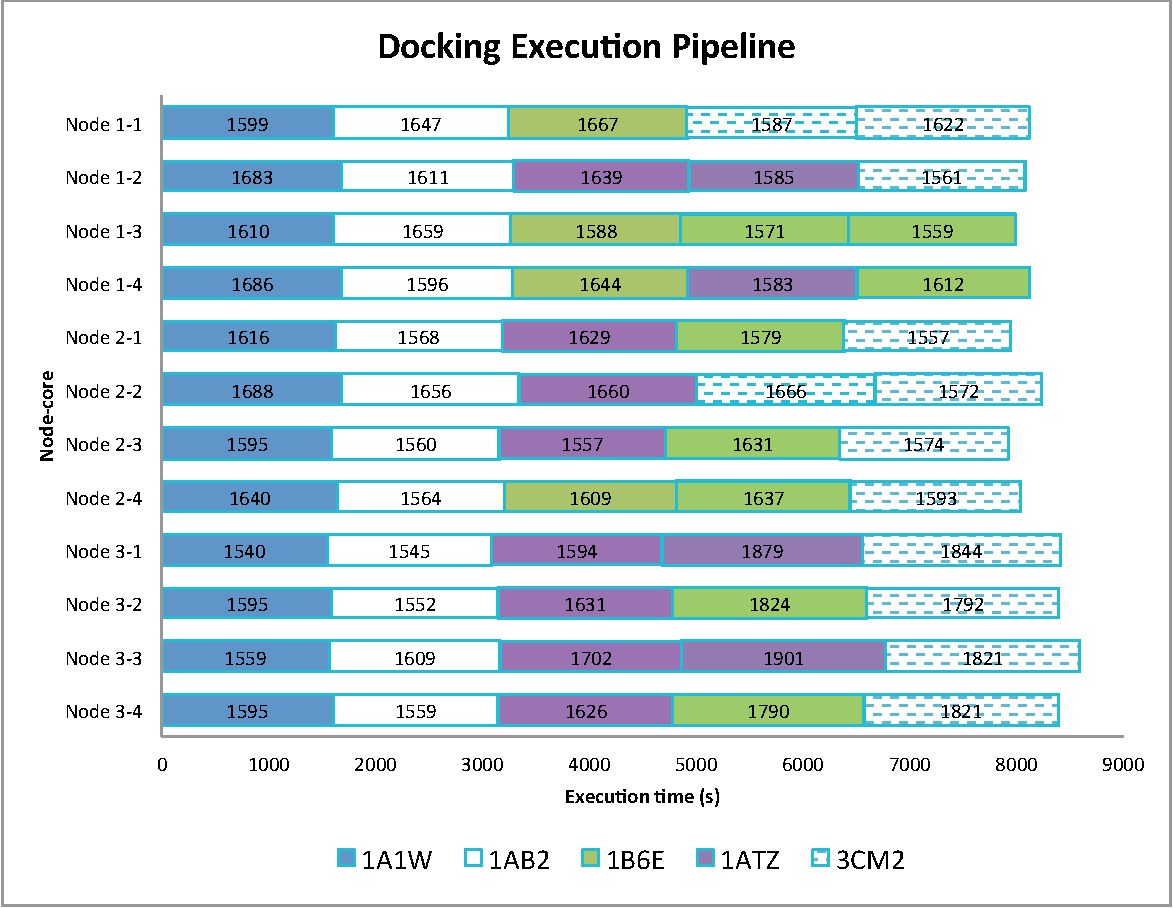
\includegraphics[width=0.5\linewidth]{images/Romain/fig8-color} 
%		\caption{Distribution de la charge lors du docking de 5 protéines (la durée de chaque exécution est indiquée dans les blocks)}\label{fig:balance}\vspace{-0.5cm}
%	\end{center}
%\end{figure} 

 
Dans un deuxième moment nous avons effectué le docking inversé du ligand X23 sur un ensemble de 100 protéines issues de la base PDB. Ici, l'utilisation du découpage a permis une  meilleure utilisation des ressources grâce à l'équilibrage de charge %(voir Figure \ref{fig:balance}) 
mais aussi meilleure prise en charge de la tolérance aux fautes. En effet, la Figure \ref{fig:performance} affiche la durée moyenne d'exécution d'une tâche selon les différentes méthodes considérées dans ce travail. Ainsi, une exécution de type blind docking nécessitait plus de 5h30, et toute interruption oblige la réexécution complète de la tâche. À l'opposé, l'interruption d'une tâche issue d'une décomposition en 12 parties ne demande qu'une demi-heure de ré-exécution, en cas de défaillance.  


 

\section{Hétérogénéité des Ressources de Calcul : adaptation de Apache Hadoop aux grids pervasifs} \label{sec:Guilherme}

La suite logicielle Apache Hadoop\footnote{\url{http://hadoop.apache.org/}} est très populaire dans le domaine du \textit{big data} et du calcul distribué. En effet, c'est l'un des outils pionniers dans le traitement de grandes masses de données grâce au support du paradigme de programmation \textit{MapReduce} \cite{Dean2008}. Bien que Apache Hadoop puisse être déployé sur des clusters composés de milliers de machines, ces ressources sont supposées être homogènes, sauf dans le cas d'une configuration spécifique de la part de l'administrateur. En effet, l'exécution des application \textit{MapReduce} dépend d'une bonne corrélation entre l'ordonnancement des tâches et les ressources alloués, or la présence de ressources hétérogènes ou dynamiques n'est pas suffisamment prise en charge par Hadoop. 

C'est pour cette raison que nous avons lancé le projet STIC-AmSud PER-MARE (Adaptive Deployment of MapReduce-based Applications over Pervasive and Desktop Grid Infrastructures - \cite{PER-MARE}) dont j'ai été l'idéalisateur et le coordinateur international. Le but de ce projet de collaboration international entre la France, le Brésil et l'Uruguay était de permettre le support aux applications \textit{big data} de type \textit{MapReduce} dans des environnements de type grid pervasif, c'est à dire, des environnements de calcul faiblement connexes marqués par l'hétérogénéité et par la volatilité des ressources \cite{3PGCIC}. Le projet PER-MARE était organisé autour de deux volets : d'un côté l'adaptation de la plate-forme Hadoop aux environnements pervasifs, et de l'autre le développement d'une solution de calcul distribué totalement répartie capable d'exécuter des applications de type \textit{MapReduce} (la plate-forme CloudFIT, traitée en section XXXX).
 %TODO mettre le lien vers la section cloudfit
 
Dans la suite de cette section on présentera donc l'architecture du framework Apache Hadoop et ses limitations concernant l'hétérogénéité des ressources. par la suite on verra les efforts effectués afin d'introduire des éléments liés au contexte dans l'ordonnancement des tâches, améliorant ainsi la performance et l'adaptabilité de la plate-forme. 



\subsection{Architecture et Ordonnancement dans Hadoop \label{subsec:ordoHadoop}}

Le framework Apache Hadoop est en réalité un écosystème assez important composé de presque une dizaine d'outils et services, allant de la gestion "bas niveau" des données et tâches de calcul à l'intégration avec des sources extérieures et le requêtage haut-niveau (parfois en imitant le langage SQL). Certains de ces outils ont été rajoutés au fil du temps grâce à des efforts de différents contributeurs (par exemple, le système de base de données HBASE développé initialement par Facebook). D'autres outils faisaient partie du projet dès son départ mais ont gagné un statut "projet" propre, comme par exemple le service ZooKeeper, responsable de la coordination distribuée fiable entre les n{\oe}uds et souvent au c{\oe}ur des efforts de tolérance aux fautes de Hadoop.

La plate-forme Hadoop elle aussi a subi des modifications au fil du temps. La version initiale (version 1.x) était extrêmement ancrée sur le paradigme \textit{MapReduce}, qui était le seul moyen d'utiliser la plate-forme. À partir de 2012 la version 2.x Hadoop devient une plate-forme plus générique, où l'on peut toujours exécuter des applications \textit{MapReduce} à côté d'autres applications. En effet, Hadoop devient surtout un gestionnaire de ressources qui aide à déployer et exécuter les tâches qui lui sont assignées.  

Au c{\oe}ur de la version 2.0 de Hadoop nous trouvons deux services principaux organisés chacun selon une architecture maître-esclave : le système de stockage distribué nommé HDFS (Hadoop Distributed File System) et le système de gestion des ressources nommé YARN (Yet Another Resource Negotiator). Les deux services présentent des composants jouant les rôles de maître ou esclave comme présenté en Figure \ref{fig:ArquiteturaHadoop} : les processus \textit{NameNode} et \textit{ResourceManager} correspondent aux rôles de maître dans HDFS et YARN, respectivement, et les processus \textit{DataNode} et \textit{NodeManager} correspondent aux parties esclaves. 

Nous pouvons observer aussi dans la Figure \ref{fig:ArquiteturaHadoop} la présence de deux autres composants appelés \textit{ApplicationMaster} et \textit{Containers} (conteneurs). L'\textit{ApplicationMaster} est un processus désigné pour effectuer l'ordonnancement des tâches de calcul d'une seule application, qui seront exécutées par des éléments \textit{Container} associés.  

\begin{figure}[!ht]
	\centering
	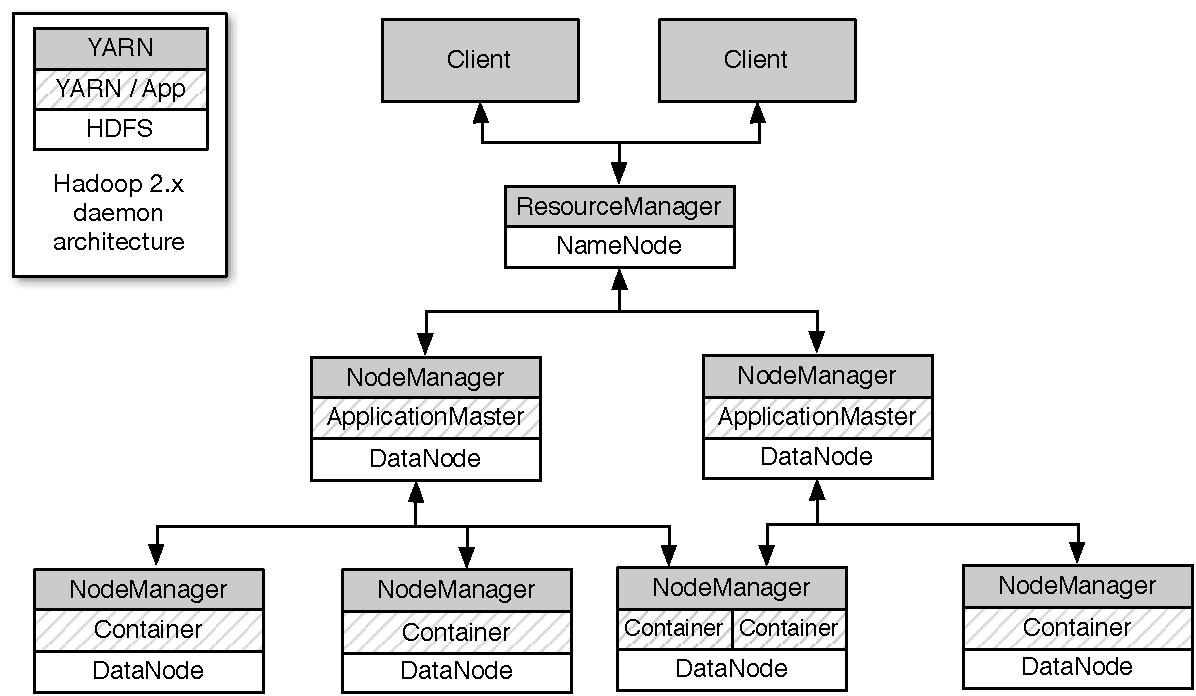
\includegraphics[width=0.85\linewidth]{img/HadoopArch.pdf}
	\caption{Architecture de base de Apache Hadoop 2.x}
	\label{fig:ArquiteturaHadoop}
\end{figure}


On observe donc que le framework Hadoop utilise deux niveaux d'ordonnancement. Les "jobs" représentent des instances avec une granularité plus grande, alors que les tâches représentent des instances de plus fin grain présentes au sein d'un job. 

L'ordonnancement au niveau des jobs est effectué par le \textit{ResourceManager}, la seule entité qui a une vue globale des ressources du système grâce aux informations envoyées par les \textit{NodeManager}. Grâce à ces informations, le \textit{ResourceManager} peut arbitrer la répartition des ressources entre les applications, en se basant sur différentes métriques telles que l'utilisation des ressources, l'équité, les contrats SLA, etc. Un \textit{ApplicationMaster} est ainsi détaché pour chaque application et devient responsable par l'ordonnancement et l'exécution des tâches de cette application par le biais des \textit{conteneurs}, des unités de calcul isolées et disposant d'un accès limité aux ressources (mémoire, CPU). 

Vu cette complexité, le \textit{ResourceManager} a été projeté de manière à pouvoir être optimisé selon contraintes et paramètres des utilisateurs, grâce à un mécanisme d'extensions. Toutefois, la plupart des utilisations répertoriées dans la littérature n'utilisent que les ordonnanceurs livrés avec Hadoop. Le plus simple de ces algorithmes d'ordonnancement est le \textit{Internal Scheduler}, une simple liste d'exécution où les jobs sont servis selon leur ordre d'arrivée (FIFO). Évidemment, cet algorithme n'est indiqué que pour les clusters où la compétition pour des ressources n'est pas un problème. 

Deux autres algorithmes sont souvent cités : l'algorithme \textit{Fair Scheduler} et l'algorithme \textit{Capacity Scheduler}. \textit{Fair Scheduler} utilise un mécanisme d'ordonnancement à deux niveaux pour effectuer un partage équitable entre des jobs de petite taille \cite{Hadoop}. \textit{Capacity Scheduler}, de son côté, a été créé pour l'utilisation de Hadoop dans un environnement où plusieurs partenaires contribuent afin de composer un grand cluster. En effet, le \textit{Capacity Scheduler} offre des garanties minimales d'accès aux ressources pour chaque partenaire, tout en permettant l'utilisation élargie du cluster lorsque des ressources se trouvent libres \cite{Hadoop}.

Les trois algorithmes cités ci-dessous illustrent des approches différentes pour la gestion des jobs, mais cela se fait uniquement par rapport à des facteurs tels que la disponibilité de ressources ou les politiques d'équité, sans jamais prendre en compte la dynamicité et l'hétérogénéité de l'environnement d'exécution. En effet, Hadoop considère que la gestion à grain fin de l'exécution incombe au  \textit{ApplicationMaster}, qui a une vue plus proche de l'application mais qui est aussi limité aux ressources que lui sont attribués au départ.

Malheureusement, le fonctionnement de l'\textit{ApplicationMaster} est peu documenté. Afin de combler ce manque d'information, nous avons analysé son code source et conduit des expériences pour comprendre ses politiques d'allocation des tâches (résultats publiés dans \cite{UBICOMM2014}). Ce que ressort est un simple mécanisme de remplissage des n{\oe}uds visant la proximité des tâches : on remplit un n{\oe}ud avec autant de conteneurs qu'il peut supporter, pour ensuite commencer re remplissage du prochain n{\oe}ud.   

Ceci nous a permis aussi d'observer que l'\textit{ApplicationMaster} se limite à répartir les conteneurs sans une véritable adéquation au contexte d'exécution. Toute connaissance sur la capacité des n{\oe}uds provient du \textit{ResourceManager}, la seule entité qui est alimentée avec ces informations. Ainsi, la modification des algorithmes d'ordonnancement dans le but d'inclure des informations de contexte doit se faire en étroite relation avec le \textit{ResourceManager}.



\subsection{État de l'Art} \label{sec:related}

La littérature propose différentes approches pour rendre Hadoop plus compatible avec les environnements hétérogènes. Des travaux comme \cite{Kumar2012}, \cite{Tian2009} ou \cite{Rasooli2012} assument que les applications \textit{MapReduce} sont exécutées régulièrement dans un environnement de "production", et que chacune des applications a des besoins spécifiques en CPU, mémoire, réseaux ou en stockage. Cette hypothèse considère donc la possibilité d'optimiser l'exécution des application en faisant la correspondance entre les besoins et les caractéristiques des ressources. De même, \cite{Isard2009} propose un algorithme d'ordonnancement où une fonction de coût basée sur un graphe "capacité-demande" permet l'ordonnancement des jobs.

Les travaux cités ci-dessus considèrent des ressources hétérogènes mais statiques et, une fois lancés, ces jobs ne sont plus "suivis" car l'environnement est supposé immuable. Une manière de rendre cet ordonnancement plus dynamique est d'incorporer des informations sur le déroulement des tâches. Par exemple, \cite{Zaharia2008} et \cite{Chen} essayent d'améliorer la distribution des tâches afin de réduire le temps de réponse dans des clusters de grande taille. Pour cela, \cite{Zaharia2008} utilise des heuristiques pour estimer la progression des tâches et ainsi décider s'il faut lancer des tâches spéculatives. Les tâches spéculatives sont des doublons (ré-soumissions) qui sont lancées lorsqu'il y a la soupçon qu'une tâche originale est retardée à cause d'un n{\oe}ud défaillant ou trop lent. Dans une ligne similaire, \cite{Chen} propose l'utilisation des traces historiques d'exécution afin d'aider cette décision. 


Une autre manière d'augmenter la performance passe par un meilleur placement des données et par l'utilisation de cette information pour le déploiement des jobs \cite{Xie2010}. En faisant un placement optimisé des données, on réduit les transferts de données occasionnés par le lancement de tâches spéculatives sur d'autres n{\oe}uds. Une approche similaire est présentée par \cite{Cavallo2015}, qui étudie les problèmes d'ordonnancement et répartition des données dans les clusters géographiquement distribués. Ainsi, ces auteurs présentent un mécanisme d'ordonnancement basé sur les ressources de calcul mais aussi sur le débit du réseau.  

Sans aucun paramètre supplémentaire, les mécanismes cités jusqu'à présent ont comme résultat un équilibrage de charge, obligeant les n{\oe}uds les plus rapides à travailler plus et les moins performants à exécuter moins de tâches. Une manière de rompre cette logique est utilisée par \cite{Sandholm2010},  qui permet d'influencer l'ordonnancement grâce à des profils d'exécution suggérés par l'utilisateur (par exemple, privilégier les n{\oe}uds lents si le job n'est pas prioritaire).  

Il faut observer cependant que la difficulté à adapter l'exécution de \textit{MapReduce} sur des environnements hétérogènes (et dynamiques) est en grand partie due à la conception même de la plate-forme Apache Hadoop, qui est très hiérarchique (voir Figure \ref{fig:ArquiteturaHadoop}). Certains travaux essayent de s'affranchir de ces barrières en développant d'autres plates-formes compatibles avec \textit{MapReduce} mais plus adaptées à l'a dynamicité des ressources.  L'utilisation de overlays P2P est ainsi un choix naturel, comme le montrent \cite{Marozzo2012} et \cite{Steffenel20151034}. Dans le système proposé par \cite{Marozzo2012}, les n{\oe}uds incarnent les différentes fonctions de l'architecture Apache Hadoop (NameNode, etc.) selon les besoins de l'application. Cependant, ce travail vise la tolérance aux fautes et n'explore pas les possibilités d'optimisation de l'ordonnancement des jobs et des tâches. 

L'approche adoptée par la plate-forme CloudFIT \cite{Steffenel20151034} est différente car même si elle repose aussi sur un overlay P2P, on n'essaye pas d'imiter le fonctionnement de Hadoop. CloudFIT est une plate-forme générique de calcul distribué, où des tâches Map et Reduce sont distribuées aux n{\oe}uds de façon opportuniste, selon un mécanisme "bag of tasks". Cette distribution est aussi guidée un ordonnancement guidé par le contexte des ressources et par des profils d'exécution fournis par les applications. Nous détaillerons le fonctionnement de CloudFIT dans le chapitre suivant.

Il faut aussi noter que, à l'exception de CloudFIT, les travaux cités précédemment ne tiennent pas compte de l'évolution des ressources au fil de l'exécution : les ressources sont décrites mais pas observées. Malgré la diversité de travaux sur l'importance de la prise en compte du contexte d'exécution \cite{Baldauf, Maamar, Ramakrishnan2014, Najar2015}, Hadoop reste essentiellement une plate-forme statique. Pour toutes ces raisons, une partie de notre travail au sein du projet STIC-AmSud PER-MARE a été d'intégrer les informations de contexte à l'exécution de Hadoop.

\subsection{Ordonnancement Orienté par le Contexte} \label{sec:desenv}

Comme indiqué dans la section \ref{subsec:ordoHadoop}, l'élément central de l'ordonnancement est le \textit{Resource Manager}. En effet, c'est grâce aux informations fournies par cet élément que les ordonnanceurs de Hadoop tels que le \textit{Capacity Scheduler} décident du démarrage et du placement des tâches. 

L'implémentation par défaut de Hadoop considère qu'un \textit{NodeManager} déclare ses ressources au \textit{ResourceManager} lors de sa connexion au réseau Hadoop, or la description de ces ressources est usuellement obtenue à partir de fichiers de configuration statiques. Afin de rendre cette information de contexte dynamique, nous devons mettre en place un mécanisme de capture de contexte et aussi permettre au \textit{NodeManager} de communiquer périodiquement ses ressources au \textit{ResourceManager}. 

Afin de modifier le moins possible le code de Hadoop, nous avons développé un module de capture de contexte qui peut être greffé à Hadoop et ainsi mettre à jour les informations sur les ressources disponibles. Les sous-sections suivantes détaillent le fonctionnement de ce module et aussi le mécanisme retenu pour son intégration à Hadoop.

\subsubsection{Le collecteur de contexte\label{sec:gestionnairecontexte}}
Par défaut, Hadoop obtient des informations sur les ressources des n{\oe}uds à partir de fichiers de configuration au format XML. Ces fichiers contiennent plusieurs paramètres, dont le nombre d'unités d'exécution (c{\oe}urs de calcul) et la capacité de la mémoire des n{\oe}uds. Une fois lues, ces informations ne sont pas mises à jour, sauf en cas de redémarrage du n{\oe}ud. Afin de rendre possible l'exécution de Hadoop dans un environnement pervasif, nous avons mis en place un mécanisme de collecte d'informations de contexte qui peut être utilisé pour ajourner la base de connaissances du \textit{ResourceManager}.

Ce collecteur de contexte a été développé dans le cadre du projet PER-MARE\cite{PER-MARE} et est structuré selon le diagramme de classes présenté en Figure \ref{fig:CollectorDiag} \cite{UBICOMM2014}. La capture des différents éléments de contexte se font grâce à l'API standard Java Monitoring API \cite{Oracle}, qui permet l'accès aux caractéristiques de la machine virtuelle Java et de la machine hôte. En effet, cela nous permet d'obtenir des informations de contexte telles que le nombre de processus (c{\oe}urs de calcul), la mémoire du système, ou la charge de ma machine. Le collecteur de contexte a été structuré avec un ensemble d'interfaces et de classes abstraites, ce qui permet de généraliser le processus de la collecte des données. De plus, en raison de sa conception, il est simple d'intégrer des nouveaux collecteurs et ainsi diversifier les informations de contexte.

\begin{figure}[!ht]
	\centering
	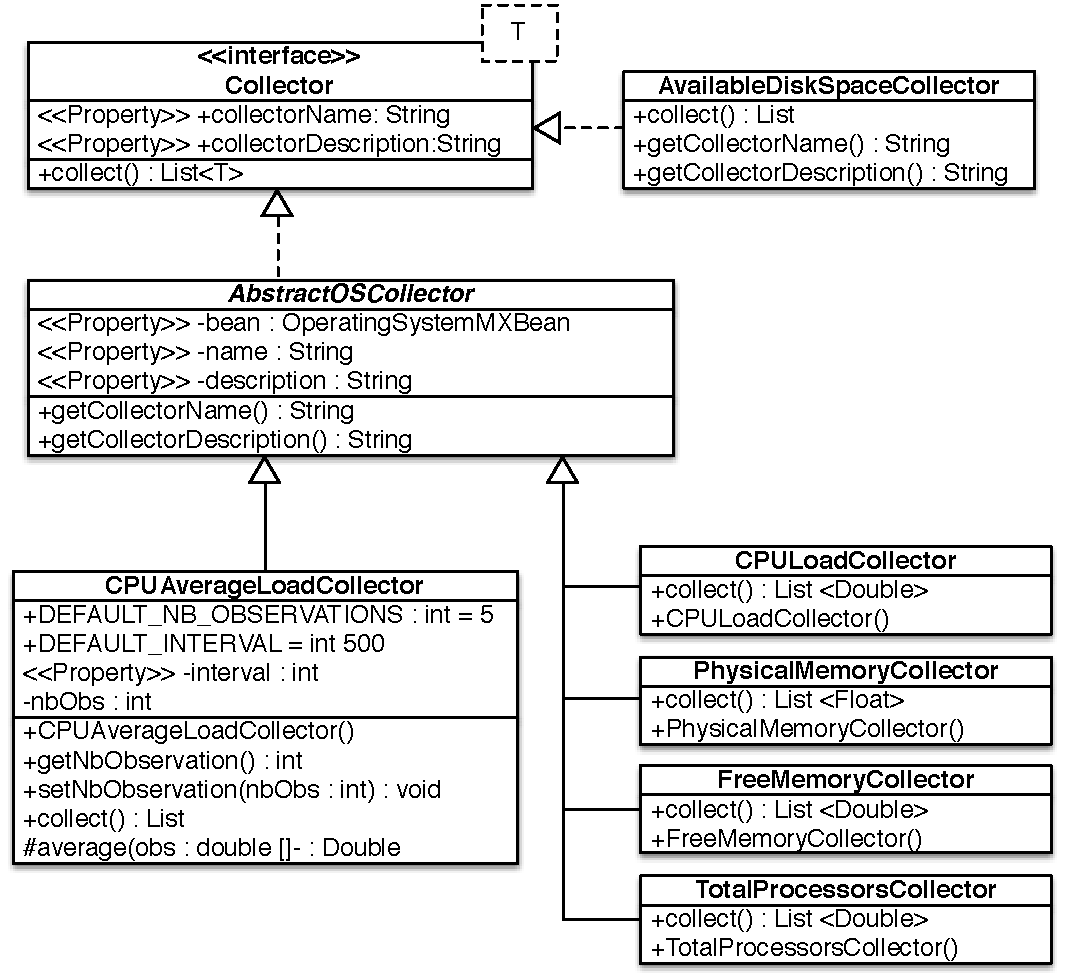
\includegraphics[width=0.75\linewidth]{img/CollectorUML2.pdf}
	\caption{Structure du collecteur de contexte}
	\label{fig:CollectorDiag}
\end{figure}

Cependant, il ne suffit pas de remplacer les fichiers de configuration XML par les informations du collecteur car ces informations resteraient statiques. Afin d'ajourner le \textit{ResourceManager}, il faut que le collecteur de contexte de chaque n{\oe}ud puisse communiquer son état au \textit{ResourceManager}, et cela à n'importe quel moment de l'exécution. Afin de rendre ceci possible, nous avons étendu les possibilités de communication entre le \textit{ResourceManager} et les \textit{NodeManager}, comme expliqué dans la section suivante.    

\subsubsection{Communication}
Dans l'architecture Hadoop, les informations de contexte collectées par les n{\oe}uds esclaves (\textit{NodeManager}) doivent être transmises au n{\oe}ud maître (\textit{ResourceManager}), qui sera en charge de l'ordonnancement. Au lieu de créer un mécanisme séparé, nous avons choisi d'intégrer cette communication au sein de l'API ZooKeeper \cite{Hunt2010}, qui fait partie de l'écosystème Hadoop. Dans notre cas, les services de ZooKeeper seront utilisés pour récupérer les informations de contexte et les rendre disponible auprès le \textit{ResourceManager}. 

\begin{figure}
	\centering
	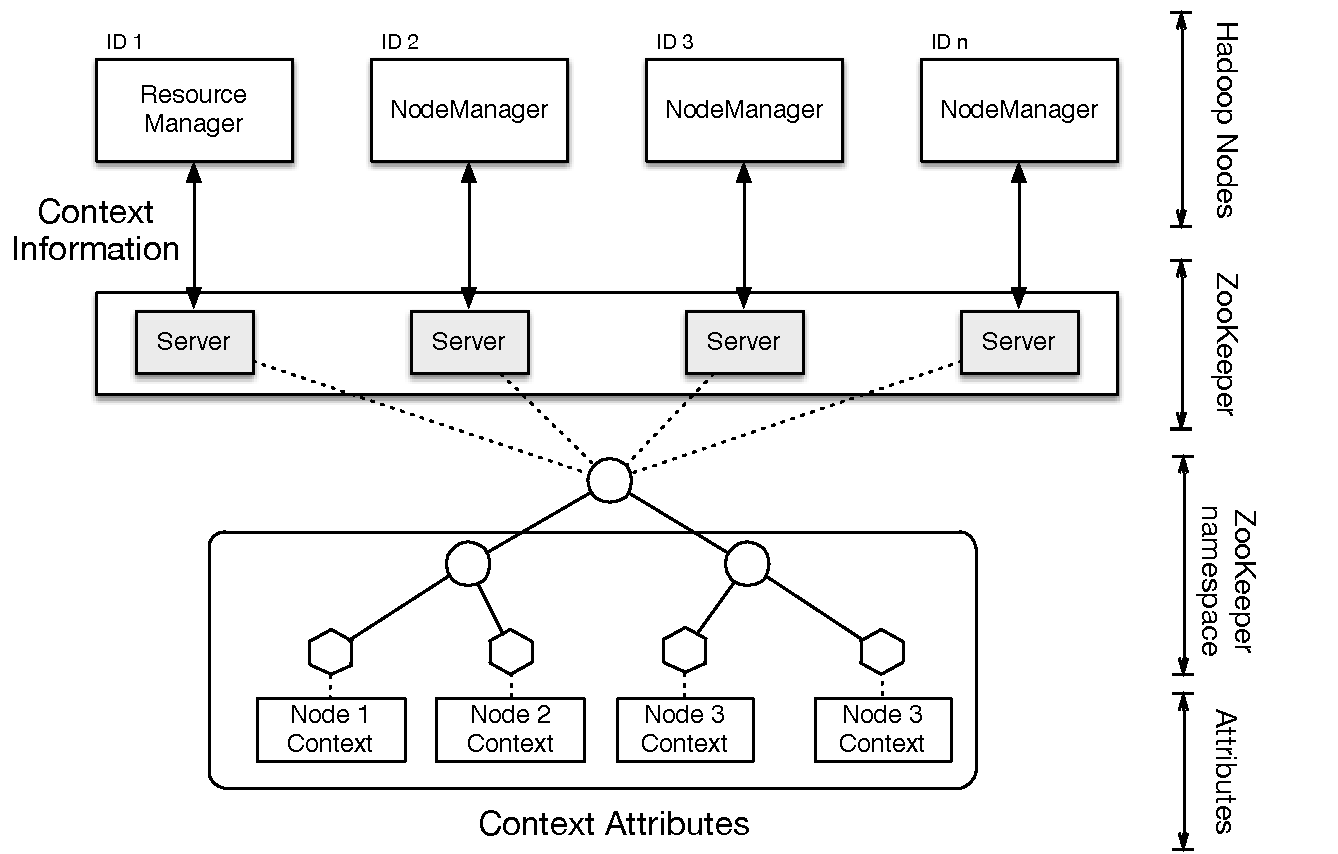
\includegraphics[width=1\linewidth]{img/Zookeeper} 
	\caption{Utilisation de ZooKeeper pour distribuer l'information de contexte\label{fig:zookeeper}}
\end{figure}


Comme illustré en Figure \ref{fig:zookeeper}, tous les esclaves (\textit{NodeManager}) exécutent une instance du service \textit{NodeStatusUpdater}, lequel collecte régulièrement les données sur la disponibilité des ressources (par exemple, à chaque 30 secondes). Si les ressources varient plus qu'un certain seuil/plafond, le tableau dans ZooKeeper sera mis à jour. Ce seuil/plafond est nécessaire car le système d'exploitation peut subir des légères variations des ressources (par exemple, la quantité de mémoire disponible) alors que ces variations n'ont pas un impact sur la capacité d'un n{\oe}ud. Ce mécanisme contribue aussi pour réduire la quantité d'informations échangées et évite trop d'événements qui pourrait impacter la performance de l'algorithme d'ordonnancement. 

De manière similaire, le maître (\textit{ResourceManager}) crée aussi un service pour surveiller les informations sur de ZooKeeper. Lorsque ZooKeeper détecte une modification des données, le maître sera notifié et pourra mettre à jour les informations utilisées par l'ordonnanceur. Les modifications apportées au code source du \textit{ResourceManager} et des \textit{NodeManager} est assez limitée, permettant son application sur différentes versions de Hadoop.

Dans la section suivante nous allons montrer les résultats de quelques expériences faites pour valider ce mécanisme.


\subsection{Évaluation Pratique} \label{sec:exper}

Afin d'évaluer l'impact de la prise en compte du contexte dans le cadre de l'ordonnancement des tâches, nous avons conduit une série d'expériences sur un petit cluster dédié. Cet environnement nous permet de contrôler les ressources disponibles et aussi ceux "observés" par le framework Hadoop, de manière à pouvoir mesurer l'impact d'une mauvaise détection et les avantages de l'adaptation au contexte. Dans les tests effectués, nous avons observé le comportement de Hadoop selon deux métriques, la ressource "mémoire disponible" et le nombre de c{\oe}urs de calcul (\textit{v-cores}). Ces paramètres sont toujours renseignés au \textit{ResourceManager} et font partie des principaux attributs utilisés par l'algorithme Capacity Scheduler. En effet, la mémoire totale disponible et le nombre de c{\oe}urs permettent la définition du nombre de tâches simultanées (conteneurs) qui peuvent être exécutées par un n{\oe}ud. Une mauvaise information peut donc créer une surcharge de la machine, affectant la performance.  

Pour la définition des scénarios d'exécution, nous avons travaillé avec l'hypothèse que la performance est dégradée si la mémoire disponible annoncée au gestionnaire de ressources est supérieure à celle réellement disponible. La situation contraire (plus de mémoire disponible que celle annoncée) n'impacte pas l'exécution d'une tâche. Ainsi, nous avons défini 4 situations d'exécution :

\begin{description}
	\item[Scénario A :] dans ce scénario "de contrôle" la mémoire disponible annoncée au gestionnaire de ressources correspond à la mémoire disponible. De même, le nombre de c{\oe}urs de calcul renseigné correspond au nombre de c{\oe}urs disponibles. Les ressources ne varient pas pendant l'exécution, ce qui peut être considéré comme le "best case". 
	\item[Scénario B :] dans ce cas, la mémoire disponible et le nombre de c{\oe}urs sont inférieurs à ceux annoncés. Cependant, elle ne sera pas mise à jour au niveau du gestionnaire de ressources, reproduisant ainsi le comportement par défaut de Hadoop. Comme l'ordonnanceur ne s'adapte pas, ceci peut être considéré comme un scénario "worst case".
	\item[Scénario C :] dans ce troisième cas, le collecteur de contexte est actif dès le départ et renseigne les ressources effectivement disponibles à chaque 30 secondes. Ainsi, quand l'application est lancée, l'ordonnanceur est au courant du contexte d'exécution et peut lancer les tâches conformément à ces ressources, sans surcharger les machines. 
	\item[Scénario D :] finalement, ce scénario représente une extension du Scénario C dans lequel l'exécution de l'application \textit{MapReduce} démarre avant la mise à jour du collecteur de contexte. De cette manière l'ordonnanceur est initialisé avec des informations incorrectes et doit s'adapter pendant l'exécution. Cette adaptation n'est pas immédiate car elle ne concerne que l'ordonnancement des tâches en attente, pas celle des tâches déjà en exécution.
\end{description}


\subsubsection{Benchmarks et environnement de test}

Deux types différents d'application ont été utilisés comme benchmarks afin de vérifier l'impact de l'adaptation au contexte. Même si les applications \textit{big data} sont fortement dépendantes de l'accès mémoire, d'autres facteurs comme l'utilisation de la CPU ou les opérations d'entrée/sortie (I/O) sont aussi importantes. Pour cela, les deux applications choisies ont des profils différents par rapport à leurs besoins en mémoire, CPU et  I/O \cite{Benchmarks}, comme indiqué ci-dessous :
\begin{itemize}
	\item TeraSort: L'application TeraSort \cite{TeraSort2008} est une application destinée à effectuer le tri d'un grand ensemble de données. C'est un benchmark très populaire car les algorithmes de tri stressent la mémoire et la CPU au même temps qu'ils sollicitent l'I/O à cause des masses des données à trier ;
	\item TestDFSIO: Le benchmark TestDFSIO a été conçu spécifiquement pour étudier l'interaction de Hadoop avec HDFS, permettant la découverte de goulots d'étranglement au niveau du réseau d'interconnexion, du système d'exploitation et de la configuration Hadoop. Dans cette application, la mémoire et la CPU sont moins sollicitées.
\end{itemize}

Les deux benchmarks font partie de la plate-forme de tests HiBench \cite{HiBench}. Le tri TeraSort a été exécuté sur un ensemble de données de 15 GB, alors que TestDFSIO a été exécuté avec 90 fichiers de 250 MB chacun. Les différents scénarios ont été exécutés sur la plate-forme Grid'5000 \cite{g5k}. Nous avons configuré un réseau dédié avec 5 machines (dont une "maître" et quatre "esclaves"), chacune avec la configuration suivante : 2 Intel Xeon CPU E5420 @ 2.50 GHz (8 c{\oe}urs par n{\oe}ud) et 8 GB de mémoire RAM. Tous les n{\oe}uds exécutent Ubuntu-x64-12.04, avec JDK 1.7 et la distribution Apache Hadoop 2.5.1. 

L'analyse des performances se fait grâce à l'étude des fichiers de log de chaque tâche (conteneur), qui contiennent des informations sur le n{\oe}ud d'allocation, le moment de démarrage et le temps nécessaire pour l'exécution de chaque tâche. Nous avons choisi d'exécuter les tâches "maître" sur un n{\oe}ud séparé afin de ne pas surcharger les n{\oe}uds esclaves avec des activités de gestion de Hadoop. 

Finalement, afin d'émuler la réduction des ressources en mémoire et c{\oe}urs de calcul nécessaires aux scénarios B, C et D, nous avons choisi de réduire le nombre effectif de n{\oe}uds utilisés, une méthode drastique mais plus fiable que la limitation logicielle des ressources disponibles.

\subsubsection{Résultats\label{sec:5.4}} 

Les exécutions des benchmarks dans les différents scénarios sont représentées par les diagrammes de Gantt des Figures \ref{fig:gantts} et \ref{fig:DFSIO}, respectivement pour TeraSort et TestDFSIO. De même, les Tableaux \ref{tab:resumo} et \ref{tab:DFSIO} résument les données clés de ces expériences, avec le temps total d'exécution des tâches \textit{map}, le temps moyen d'exécution, l'écart type, le nombre de tâches \textit{map} et aussi le nombre de tâches spéculatives démarrées.  

\begin{figure*}[!ht]
	\centering
	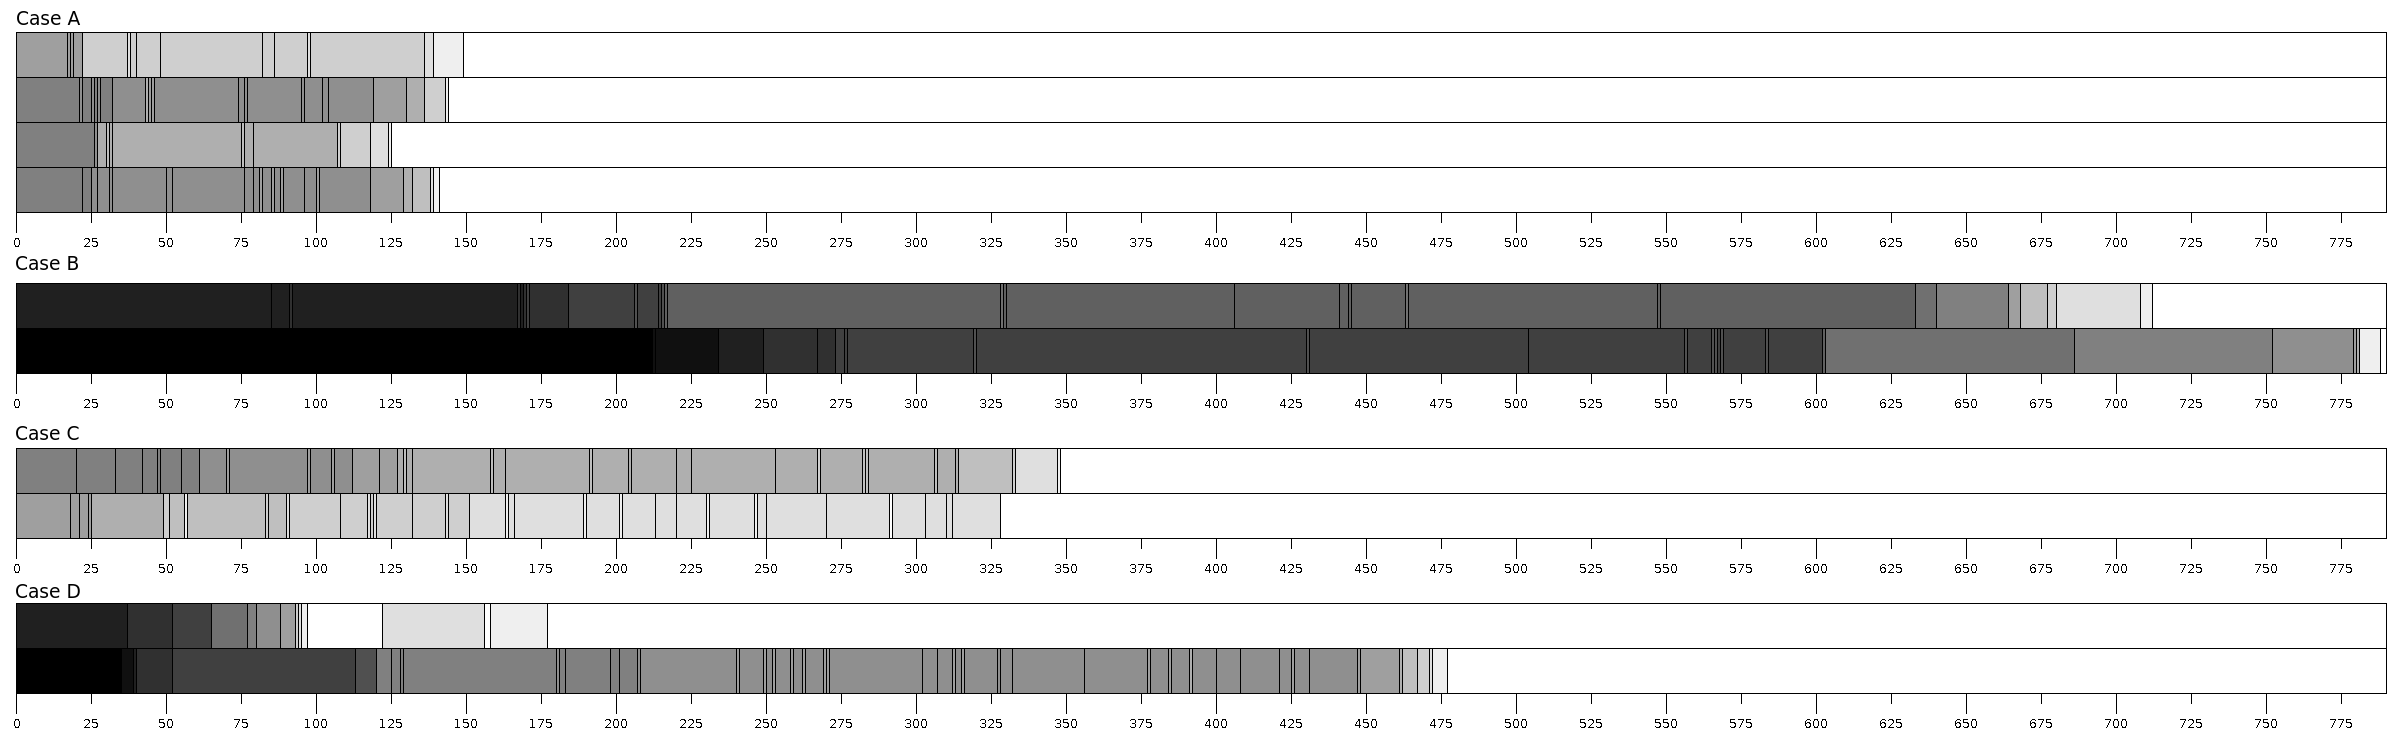
\includegraphics[width=1\textwidth]{img/todos}
	\caption{Diagramme de Gantt pour l'exécution de TeraSort}
	\label{fig:gantts}
\end{figure*}

\begin{figure*}[!ht]
	\centering
	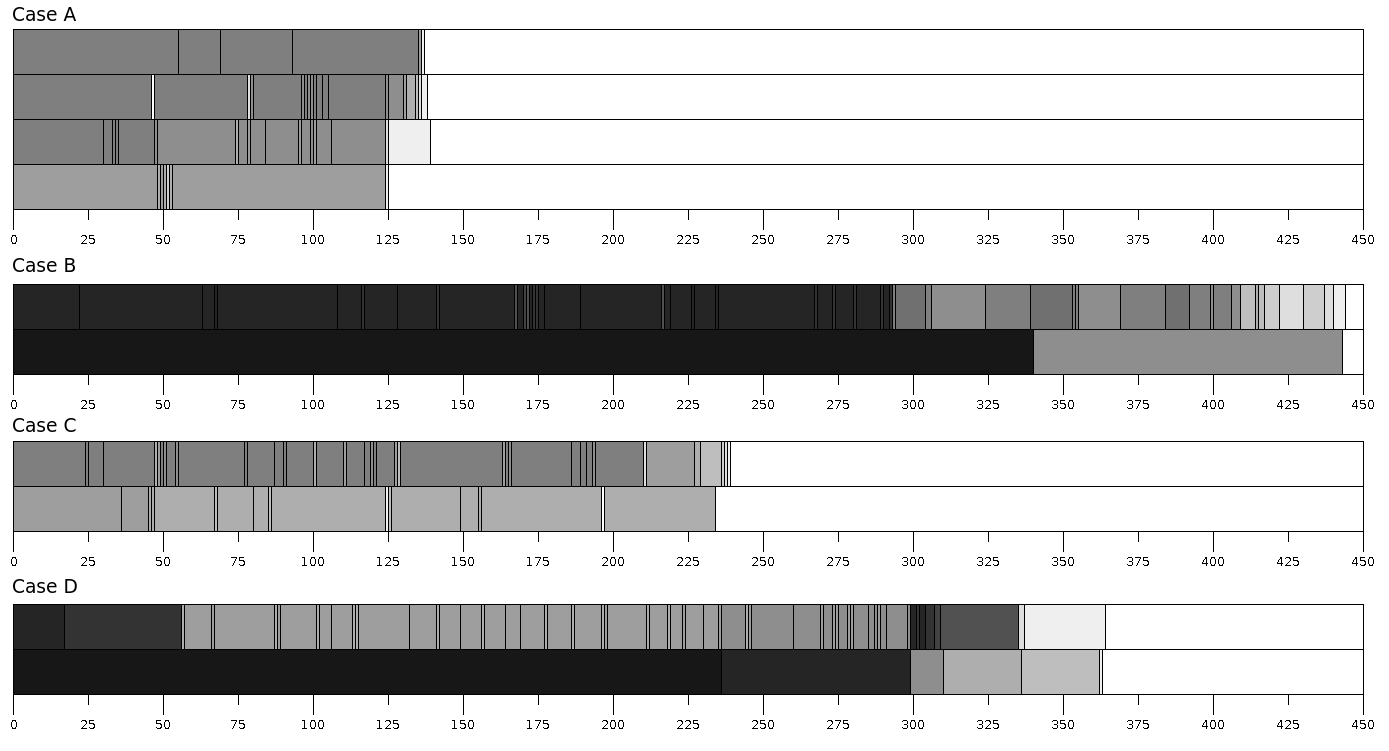
\includegraphics[width=1\textwidth]{img/todos-DFSIO}
	\caption{Diagramme de Gantt pour l'exécution de TestDFSIO}
	\label{fig:DFSIO}
\end{figure*}


\begin{table}
	\caption{Tableau récapitulatif de l'exécution de TeraSort} \label{tab:resumo}
	\centering
	\begin{tabular*}{0.6\hsize}{lllll} 
		\textbf{Scénario} & \textbf{A} & \textbf{B} & \textbf{C} & \textbf{D}\\
		\hline
		Temps total \textit{map} ({\it{s}}) & 149 & 788 & 348 & 477 \\
		Temps moyen ({\it{s}}) & 39.47 & 222.97 & 38.38 & 68.42 \\
		Écart type & 15.73 & 59.86 & 18.09 & 29.91 \\
		\# tâches \textit{map} & 76 & 76 & 76 & 76 \\
		\# tâches spéculatives & 2 & 1 & 3 & 1 \\
	\end{tabular*}
\end{table}

\begin{table}
	\caption{Tableau récapitulatif de l'exécution de TeraSort} \label{tab:DFSIO}
	\centering
	\begin{tabular*}{0.6\hsize}{lllll} 
		\textbf{Scénario} & \textbf{A} & \textbf{B} & \textbf{C} & \textbf{D}\\
		\hline
		Temps total \textit{map} ({\it{s}}) & 139 & 444 & 239 & 364 \\
		Temps moyen ({\it{s}}) & 38.95 & 85.01 & 32.20 & 81.62 \\
		Écart type  & 17.20 & 69.08 & 8.30 & 73.60 \\
		\# tâches \textit{map} & 90 & 90 & 90 & 90 \\
		\# tâches spéculatives & 0 & 9 & 0 & 1 \\
	\end{tabular*}
\end{table}


Pour les diagrammes de Gantt, chaque scénario est composé de 2 ou 4 lignes correspondant au nombre de n{\oe}uds utilisés. Comme indiqué précédemment, les scénarios B, C et D n'utilisent que la moitié des n{\oe}uds du scénario A afin de simuler la réduction des ressources. L'échelle de couleurs présent dans chaque ligne indique la surcharge des n{\oe}uds : plus sombre est le créneau, plus de conteneurs s'exécutent simultanément. De cette manière, un créneau "blanc" n'a aucun conteneur en exécution, alors qu'un créneau "noir" en contient 16 conteneurs (le double de la capacité d'un n{\oe}ud). Les séparations des créneaux indiquent soit le démarrage d'une tâche, soit une fin d'exécution, mais ne permettent pas de suivre le temps d'exécution d'une tâche précise. 

L'analyse des tableaux permet d'identifier certaines tendances. En effet, toutes les exécutions présentent un motif similaire quand on observe le temps total d'exécution : le scénario A est toujours le plus rapide, suivi de des cas C et D puis finalement  B. Nous observons aussi que les scénarios A et C ont les plus petits temps moyens et les plus petites variations de performance, indépendamment de l'application. Ceci s'explique par le fait que dans ces deux scénarios les n{\oe}uds ne sont jamais surchargés car l'ordonnanceur a des informations précises au moment du démarrage de l'application. Ceci s'observe aussi par la tonalité des créneaux, indiquant un nombre moins important de tâches en simultané. Le temps total d'exécution du scénario C est aussi deux fois plus important que celui du scénario A, une conséquence attendue à cause de la réduction des ressources. 

L'analyse du nombre de tâches spéculatives apporte aussi quelques renseignements. Dans le cas de TeraSort, tous les scénarios se comportent de manière similaire. Par contre, dans le cas de TestDFSIO le déploiement de tâches spéculatives ne se fait que lorsque le système est surchargé (notamment dans le scénario B). La raison pour cette différence vient des facteurs qui sont liés au lancement de tâches spéculatives : une tâche spéculative n'est lancée que seulement après le lancement de toute autre tâche "originale", et déclenchée seulement lorsque ces tâches sont en exécution depuis un certain temps (au moins une minute) et n'ont pas progressé autant que la moyenne des autres tâches du job. Dans le cas de TeraSort, les tâches dépendent autant de la mémoire que de la CPU et de l'I/O, et le recouvrement de ces besoins compense d'une certaine manière le manque d'une ressource. TestDFSIO, à l'opposé, s'appuie sur des ressources plus spécifiques et est donc plus enclin à la surcharge des n{\oe}uds. Et même dans les scénarios surchargés, l'utilisation d'un mécanisme de détection du contexte sur le scénario D permet à l'ordonnanceur de lisser la charge lors de la mise à jour des informations sur les ressources.

%Concerning the execution flow, as illustrated by the Gantt charts, it is possible to note that both cases B and D have a dark tone at the beginning, meaning that 16 containers are running (twice the real capacity). Also, the first containers took 20 to 50 seconds to complete execution in scenarios A and C in all experiments (cf. the first segment line). On the opposite side, during most of scenario B (and to a lesser extent D) 70 or more seconds are required, evidencing an overload on the nodes. The exception here is the TestDFSIO scenarios B and D, which have segment lines at about 25 seconds. Through further analysis, it is possible to note that all TestDFSIO experiments had at least one segment line near the 25 seconds mark, meaning this was a task very easily processed and somehow not affected by the node overload.

%Although both B and D scenarios had the same initial conditions (50\% available resources and 100\% reported resources), case D took less time to complete in all experiments (20\% to 40\% faster than B). The reason for this is that the context collector updates the reported resources in D, allowing the scheduler to reorganize tasks after the first tasks complete. This behavior is easily noted on TeraSort and TestDFSIO charts. Indeed, all D scenarios had high concentration of executing containers at the start of the job but lessened the load over time, while B scenarios had the nodes overloaded until the end due to the absence of updated information. Although the scheduler does not preempt excess containers, it is possible to observe a performance improvement of about 40\% on TeraSort and 20\% on TestDFSIO experiments as the scheduler avoids overloading the nodes.

Il faut aussi pointer un détail concernant les diagrammes de Gantt. Dans tous les benchmarks il y a un n{\oe}ud qui semble moins chargé que les autres. Ceci n'est pas la faute à une mauvaise répartition de la charge mais plutôt à la présence de tâches \textit{reduce}, qui ne sont pas affichées dans les diagrammes. En effet, Hadoop permet le démarrage de tâches \textit{reduce} aussitôt un certain nombre de tâches \textit{map} a été complété, ce qui est le cas pour ces applications.

Le résultat de ces expériences démontre que l'utilisation d'un mécanisme de collecte et de mise à jour des informations de contexte permet l'adaptation de l'ordonnanceur Hadoop aux aléas d'une plate-forme d'exécution dynamique. La solution que nous avons proposé dans ce travail permet non seulement un gain de performance dans les scénarios avec risque de surcharge mais aussi impose très peu de modification au niveau du code source de Hadoop, rendant la solution suffisamment générique et intégrable aux différentes versions de ce framework. 


\section{Bilan et Perspectives} \label{sec:disc}

%TODO rajouter une note sur le travail avec Javier et Matias, après tout ça fait partie des choses faites avec Hadoop







